\chapter{Introduction}

A \emph{recommender engine}, or just \emph{recommender}, is a system which suggests useful items to a user -- usually on a website. A user is typically assisted in their search process to find the right items. Recommender engines are able to personalise this process so that they try to suggest only items relevant for the given user. In order to do this, recommender engines rely on multiple techniques, notably \emph{collaborative filtering} and \emph{content-based filtering}.

Recommender engines are usually tightly coupled to the application they are used in. Bespoke  engines may be very dependent on the data model as well as technical constraints of those applications such as programming languages and database management systems. The adaptation of recommender engines requires knowledge and expertise in both the application and recommender engines. That effort would also add more complexity and dependencies to those applications, which are probably complex themselves, making change very expensive and time consuming. Being tightly coupled, a recommender engine is very likely to be incompatible for another application.

This project aims to develop and evaluate a framework for integrating recommender engines into applications in a loose-coupled approach which promotes amongst others reusability and is easy to integrate. In order to demonstrate those capabilities, two recommender engines -- each implementing a fundamentally different recommendation technique -- are implemented. Moreover, the framework and these recommender engines are then integrated into a complex e-commerce web application.

\section{Background Research}

\citet{ricci11} write that traditional recommendations can be observed in various scenarios, such as a peer's recommendation when buying a book or reviews when choosing a movie. The authority of the recommender has an important role in the acceptance of a recommendation. A renowned film critic may appear more credible than a random colleague whereas when it comes to car parts, a mechanist may be a the first person to ask.

With the growth of the Internet, the amount of information available on the Web increased rapidly. Especially, major e-commerce Web sites were extending their range of products and services. Although a wider and varied range of items is initially good for customers, they found it more and more difficult to find appropriate items and make the right choices of what to buy. Web sites have deployed different type of solutions -- such as search engines and more user-friendly interfaces -- to cope with this problem.

Another approach is recommender engines, which basically provide a bespoke, personalised collection of items with the intention to highlight only relevant items to a user. Depending on the recommendation technique used, various data sources are taken into account such as the user's context or previous interactions. Most recommender engines concentrate on guiding the user towards novel, unexperienced items \cite{herlocker04}.

\subsection{Problems of a Tightly Coupled Architecture}
\label{intro-bg-problems}

Throughout this report, \emph{domain applications} refer to existing software systems primarily developed for a specific organisation or application, secondarily planning to make use of recommendations and integrate recommender engines. The definition highlights the fact that these applications are usually built on extensive domain knowledge. Efforts to use recommendations either require domain savvy engineers to gain a recommendation background or recommendation savvy engineers to grasp the domain knowledge. This makes changes very difficult, time consuming and expensive. If recommender engines are tightly coupled to the same database as the domain application, changes to the data and schema may affect both applications regardless of which system applied that change.

The technology stack -- the collection of all technologies used within a software system -- is mostly tailored to the requirements of those applications and may not be the first choice for recommendation requirements. Furthermore, the best suitable technology stack may differ substantially among recommender engines themselves.

Tightly coupled software is also difficult to reuse. If an additional domain application needs to access and contribute to recommendations, a significant amount of work would be required to refactor the main application to accommodate that. Another possible case is that an organisation wants to use the recommender in another, unrelated domain.

\subsection{Recommender Techniques}
\label{intro-bg-tech}

In the course of research in this field different techniques to compute recommendations emerged. Fundamentally, techniques are classified by the information sources they rely on. The sources of personalised recommendations are typically user-item interactions (\emph{collaborative filtering}), item features (\emph{content-based filtering}), user features (\emph{demographic filtering}) as well as specialised knowledge about the user and item (\emph{knowledge-based filtering}).  Amongst those, the techniques collaborative and content-based filtering are explained as they are used by the recommender engines implemented as part of this project:

\subsubsection{Collaborative Filtering}
\label{intro-bg-tech-collaborative}

\begin{figure}[ht]
    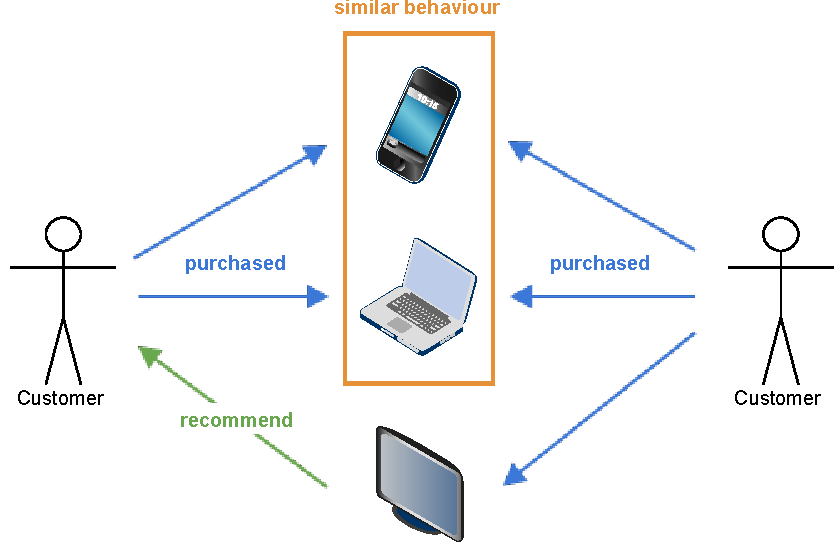
\includegraphics[width=0.7\textwidth,center]{intro/background/collaborative.pdf}
    \caption{Collaborative Filtering Diagram}
    \label{fig:intro-techniques-collaborative}
\end{figure}

This technique recommends items other users with similar preferences have shown a positive expression e.g. \emph{liked} or \emph{purchased} for before. In order to do this, the recommender engine needs to observe behaviour patterns and interactions of users. Based on these learnings, it will then look up other users with similar behaviour patterns and compute recommendations from their preferences -- preferably items that the given user -- the user the recommendations are for -- has not experienced yet.

The major advantage of this approach is that the recommender engine does not require any knowledge about the items themselves.

Figure \ref{fig:intro-techniques-collaborative} illustrates a scenario where a customer has purchased several items in the past. The recommender engine understands that the given customer is similar to other customers, as both have purchased the same phone and laptop. Then, the system computes items these similar customers purchased but the given customer has not yet. It therefore recommends a TV to the given customer.

\subsubsection{Content-Based Filtering}

\begin{figure}[ht]
    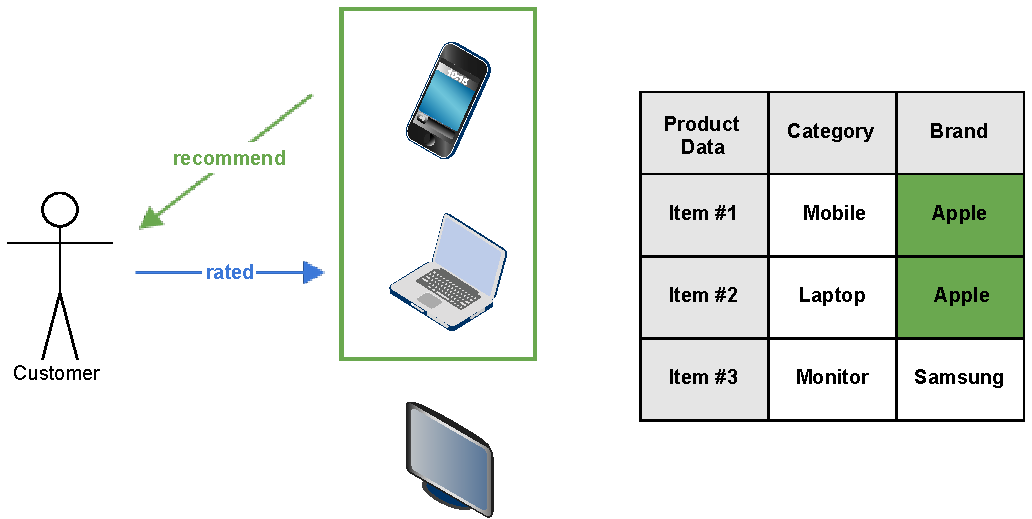
\includegraphics[width=0.7\textwidth,center]{intro/background/contentbased.pdf}
    \caption{Content-Based Filtering Diagram}
    \label{fig:intro-techniques-contentbased}
\end{figure}

Content-based recommendation methods compare item features to find similar items. Based on items the user has shown a preference for before -- such as \emph{rated} or \emph{purchased} -- other similar items are looked up based on features of this item. Figure \ref{fig:intro-techniques-contentbased} illustrates a customer who has rated an item positively. The recommender engine compares the rated item with other items, finds another item, which has the same brand and therefore recommends that item.

Demographic filtering is a specialisation of content-based filtering putting emphasis on user rather than item features. A very basic demographic filtering can be achieved by regular content-based recommender engines by sourcing user data as items. The content-based recommender engine, implemented as part of this project does not distinguish between users and items, thus is able to handle demographic queries as well.

\subsubsection{Hybrids}
\label{intro-bg-tech-hybrid}

Hybrid recommender engines make use of two or more individual recommender engines -- hereinafter referred to as components. This is in particular interesting as it enables hybrid engines to utilise different kind of filtering techniques at once. A possible motivation of using hybrid engines is to overcome weaknesses of one engine with another. However it is also possible to combine systems implementing the same technique but e.g. using different data sources.

There are many possible ways of combining techniques, which are outlined in the proposal. In this project, a \emph{weighted} hybrid recommender engine is implemented which combines the scores of its components using a linear formula. A score is a numerical preference rank attached to recommendations.

\section{Objectives}
\label{intro-objectives}

The primary objective of this project is to develop an integration framework for recommender engines whereas the secondary objectives are the development of a collaborative and a content-based recommender engine as well as the exemplified integration of framework and recommender engines into an existing, complex web application. These secondary objectives are important to provide concrete findings for the evaluation of the primary objective.

\subsection{Development of an Integration Framework}
\label{intro-objectives-framework}

As mentioned, the primary objective of this project is the development of an framework for integrating recommender engines into any domain application. The framework should have the following properties:

\begin{description}
    \item[Multi-purpose] The framework should cope with different kind of data as well as recommendation techniques.
    \item[Easy to integrate] First, the integration into a domain application should be as easy and compact as possible. Second, setting up and integration of recommender engines should be simple as well.
    \item[Non-restrictive] The usage of the framework should not restrict the capabilities of a recommender engine.
    \item[Encapsulated] Internals of domain applications and recommender engines should not be visible to each other.
    \item[Reusable] Recommender engines should be reusable. A domain application should be able to switch to another recommendation engine with minimal effort. Other recommenders shall be able to use recommendations from another recommender engine \cite{manouselis07}.
    \item[Technologically unbiased] The framework should work with any technology.
\end{description}

\subsection{Development of Two Distinct Recommender Engines}
\label{intro-objectives-engines}

In order to validate that the framework implements the aforementioned properties, two recommender engines, fundamentally different in their approaches, are to be developed -- namely a collaborative recommender (as described in \ref{intro-bg-tech-collaborative}) and a content-based recommender (as specified in \ref{fig:intro-techniques-contentbased}).

Although they are going to be used with the framework, they should be designed to be fully functional, standalone recommender engine. Their algorithmic correctness and practicality shall be reviewed in the evaluation. At the same time, the focus of this project is on the development of the framework. This means that these recommender engines may be somewhat simplified.

\subsection{Integration Into a Demo Application}
\label{intro-objectives-demo}

This objective is in particular relevant as it is a practical application of the rather theoretical framework and recommender engines. Whereas the recommender engines may be somewhat simple, it is important that the demo application is complex enough to be a good example for an integration. Henceforth, an existing, open-source e-commerce application shall be used as demo application.

This objective is going to contribute significantly to the evaluation of the ease of integration property of the framework. The size and complexity of the integration source code are a good indicator in this case.

\section{Structure of the Report}

\begin{description}
    \item[Chapter 2] illustrates the architecture and concepts of various systems of the project.
    \item[Chapter 3] goes into detail and describes the implementation, testing and technology choices.
    \item[Chapter 4] evaluates the project against the project objectives.
    \item[Chapter 5] reflects on the project outcome and possible future work.
    \item[Appendix A] contains the bibliographical references of the report.
    \item[Appendix B] offers user manuals of the various systems implemented.
    \item[Appendix C] lists the source code written for this project.
\end{description}